\documentclass{article}
\usepackage[utf8]{inputenc}
\usepackage{graphicx}
\usepackage{listings}
\title{Information System - Lab work 8}
\author{Tran Thi Hong Hanh}
\date{10 November 2017}

\begin{document}

\maketitle
\section{Requirement}
A Non-Government Organization (NGO) wants to prepare a database for all its
projects. It has diverse head offices in several countries which take manage and coordinate the projects of that country.\\
On head offices, an identifier, the city and country where it is located, its address, a phone number and the name of the director are stored. Every head office manages a set of projects, with a code, a title, dates of beginning and end, the assigned budget and the name of the person in charge. One project is formed by a set of actions that can affect to several cities.\\
We want to know what actions are realised in each city, storing its name, country and no of inhabitants. We also need an identifier to differentiate them. Also there is wished the investment of the project that corresponds to the city and a small description of the action.

\section{Design Database}
\subsection{Determine concepts that needs to be stored}
\begin{itemize}
	\item Head\_Office
	\item Projects
	\item Actions
	\item Cities
	\item Directors
\begin{figure}[h]
\centering
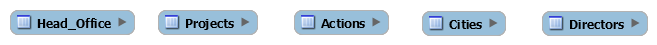
\includegraphics[scale = 0.5]{1.PNG}
\caption{Concepts}
\end{figure}
\end{itemize}
\subsection{Determine attributes of each concept}
\begin{itemize}
	\item Head\_Office(HO\_id, address, phone\_no)
	\item Projects(code, title, from\_date, to\_date, budget)
	\item Actions(action\_id, name, wished\_investment, description)
	\item Cities(city\_id, name, country, no\_of\_habitants)
	\item Directors(id, name, gender, email, address)
\begin{figure}[h]
\centering
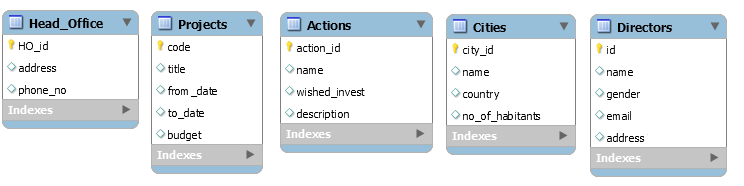
\includegraphics[scale = 0.9]{2.PNG}
\caption{Attributes}
\end{figure}
\end{itemize}

\subsection{Determine links (relationships) between them}
\begin{itemize}
	\item Head\_Office and Directors ("in charge")
	\item Head\_Office and Cities ("situated in")
	\item Projects and Actions ("have")
	\item Directors and Projects ("in charge")
	\item Actions and Cities ("implement")
	
	
\end{itemize}
\subsection{Determine types of each concept attribute}
\begin{itemize}
	\item Head\_Office
	\begin{itemize}
		\item HO\_id INT
		\item address VARCHAR(100)
		\item phone\_no INT
	\end{itemize}
	\item Projects
		\begin{itemize}
		\item code INT
		\item title VARCHAR(50)
		\item from\_date DATE
		\item to\_date DATE
		\item budget INT
	\end{itemize}
	\item Actions
		\begin{itemize}
		\item action\_id INT
		\item address VARCHAR(50)
		\item wished\_invest INT
		\item description VARCHAR(250)
	\end{itemize}
	\item Cities
		\begin{itemize}
		\item city\_id INT
		\item name VARCHAR(45)
		\item country VARCHAR(45)
		\item no\_of\_habitants INT
	\end{itemize}
	\item Directors
		\begin{itemize}
		\item id INT
		\item name VARCHAR(45)
		\item gender ENUM("M","F")
		\item email VARCHAR(50)
		\item address VARCHAR(100)
	\end{itemize}
\begin{figure}[h]
\centering
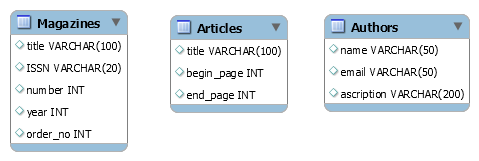
\includegraphics[scale = 0.55]{3.PNG}
\caption{Type of attributes}
\end{figure}
\end{itemize}

\subsection{Solve foreign key links}
\begin{itemize}
	\item Head\_Office
	\begin{itemize}
		\item HO\_id INT
		\item address VARCHAR(100)
		\item phone\_no INT
		\item Cities\_city\_id INT
	\end{itemize}
	\item Projects
		\begin{itemize}
		\item code INT
		\item title VARCHAR(50)
		\item from\_date DATE
		\item to\_date DATE
		\item budget INT
		\item Directors\_id INT
	\end{itemize}
	\item Actions
		\begin{itemize}
		\item action\_id INT
		\item address VARCHAR(50)
		\item wished\_invest INT
		\item description VARCHAR(250)
		\item Projects\_code INT
		\item Cities\_city\_id INT
	\end{itemize}
	\item Cities
		\begin{itemize}
		\item city\_id INT
		\item name VARCHAR(45)
		\item country VARCHAR(45)
		\item no\_of\_habitants INT
	\end{itemize}
	\item Directors
		\begin{itemize}
		\item id INT
		\item name VARCHAR(45)
		\item gender ENUM("M","F")
		\item email VARCHAR(50)
		\item address VARCHAR(100)
		\item HO\_id INT
	\end{itemize}
\begin{figure}[h]
\centering
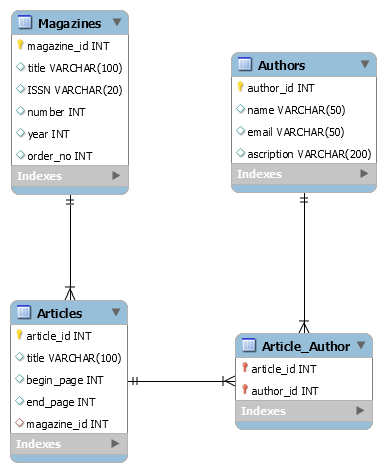
\includegraphics[scale = 0.6]{4.PNG}
\caption{Solve foreign key links}
\end{figure}
\end{itemize}
\newpage
\subsection{Implementation}
\begin{lstlisting}{showstringspaces=false}[language=SQL]
CREATE DATABASE NGO1;
USE NGO1;

CREATE TABLE Cities (
  city_id INT NOT NULL,
  name VARCHAR(45) ,
  country VARCHAR(45) ,
  no_of_habitants INT ,
  HO_id INT NOT NULL,
  PRIMARY KEY (city_id)
);

CREATE TABLE Head_Office (
  HO_id INT NOT NULL,
  address VARCHAR(100),
  phone_no INT,
  Cities_city_id INT,
  PRIMARY KEY (HO_id),
  FOREIGN KEY (Cities_city_id)
  REFERENCES Cities(city_id)
);


CREATE TABLE Directors (
  id INT NOT NULL,
  name VARCHAR(45),
  gender ENUM('M', 'F'),
  email VARCHAR(50),
  address VARCHAR(100),
  HO_id INT NOT NULL,
  PRIMARY KEY (id, HO_id),
  FOREIGN KEY (HO_id)
  REFERENCES Head_Office(HO_id)
);


CREATE TABLE Projects (
  code INT NOT NULL,
  title VARCHAR(50),
  from_date DATE,
  to_date DATE,
  budget INT NULL,
  Directors_id INT NOT NULL,
  PRIMARY KEY (code),
  FOREIGN KEY (Directors_id)
  REFERENCES Directors(id)
);


CREATE TABLE Actions (
  action_id INT NOT NULL,
  name VARCHAR(50),
  wished_invest INT,
  description VARCHAR(250) NULL,
  Projects_code INT NOT NULL,
  Cities_city_id INT NOT NULL,
  PRIMARY KEY (action_id),
  FOREIGN KEY (Projects_code)
  REFERENCES Projects(code),
  FOREIGN KEY (Cities_city_id)
  REFERENCES Cities(city_id)
);
    
\end{lstlisting}
\begin{figure}[h]
\centering
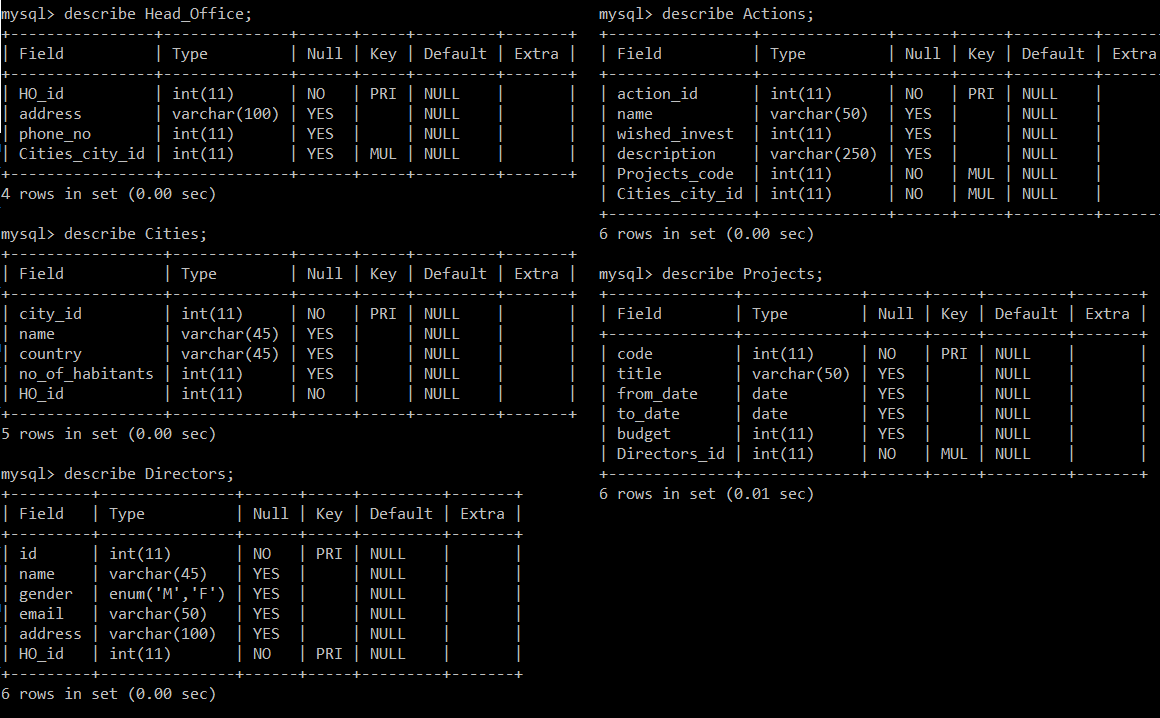
\includegraphics[scale = 0.55]{5.PNG}
\caption{Output}
\end{figure}

\end{document}
